\documentclass[11pt]{article}
\usepackage[a4paper,margin=25mm]{geometry}
\usepackage[T1]{fontenc}
\usepackage{lmodern,amsmath,amssymb,amsthm,booktabs,tabularx,tikz}
\usetikzlibrary{arrows.meta,positioning}
\usepackage[hidelinks]{hyperref}
\newtheorem{theorem}{Theorem}
\newtheorem{proposition}[theorem]{Proposition}
\newtheorem{corollary}[theorem]{Corollary}
\theoremstyle{remark}\newtheorem{remark}[theorem]{Remark}
\newcommand{\dd}{\,\mathrm d}
\newcommand{\R}{\mathbb R}
\title{A Local Smooth Transcritical Continuation Theorem\\
for the Coupled Annular Saint--Venant--Exner System}
\author{Research proof and reproducible verification record}
\date{1 November 2026}
\begin{document}
\maketitle

\noindent\textbf{Result and scope.}
For the precise coupled model below, a nondegenerate saddle condition at a
radial hydraulic critical point gives exactly two local $C^1$ profile germs.
Both are smooth, cross the critical locus, and reconstruct classical solutions
of all four original Cartesian equations. An explicit continuous parameter
family satisfies the condition. The invariant class is obtained after solving
a declared point-symmetry determining problem and constructing its quotient;
it is not an input profile ansatz to that computation. The proof concerns this
derived invariant class. It does not claim a maximal Lie algebra, arbitrary
two-dimensional data, a global boundary connection, a numerical error bound,
or literature priority. Standard stable-manifold theory is explicitly credited.

\section{Specified model, units and solution class}
Let $\mathbf w=(u,v)$, $\mathcal J(u,v)=(-v,u)$, $g,K,G>0$, and $f$ constant.
The equations are exactly
\begin{align}
E_h&:=h_t+\nabla\cdot(h\mathbf w)=0,\label{eq:mass}\\
\mathbf E_w&:=\mathbf w_t+(\mathbf w\cdot\nabla)\mathbf w
 +g\nabla(h+B)+f\mathcal J\mathbf w=\mathbf0,\label{eq:mom}\\
E_B&:=B_t+\nabla\cdot\mathbf q=0,\qquad
\mathbf q=K|\mathbf w|^2\mathbf w-G|\mathbf w|^2\nabla B.\label{eq:bed}
\end{align}
Here $B$ is an evolving bed elevation, not a prescribed topography. Any constant
porosity factor is already absorbed into $\mathbf q$. The proof requires
$h>0$ on its local spatial domain. A classical solution means that all
derivatives in these equations exist continuously; in particular the bed is
twice spatially differentiable. No entropy or weak-solution statement is used.

To fix units before specifying numerical constants, choose $L_0,H_0,U_0>0$,
put $T_0=L_0/U_0$, and scale $\mathbf x=L_0\mathbf x_*$,
$t=T_0t_*$, $(h,B)=H_0(h_*,B_*)$, $\mathbf w=U_0\mathbf w_*$,
$\mathbf q=H_0U_0\mathbf q_*$. The same system results with
\[
g_*=\frac{gH_0}{U_0^2},\quad f_*=\frac{fL_0}{U_0},\quad
K_*=\frac{KU_0^2}{H_0},\quad G_*=\frac{GU_0}{L_0}.
\]
A bed-drift rate scales as $c_*=cL_0/(H_0U_0)$. The mathematical arguments
below apply in either consistent set of units; the explicit all-one parameter
example is dimensionless. It is a constructed mathematical example, not a
calibration or an observed river flow. A physical shallow-water or mild-slope
assessment would additionally require the dimensional scales and closure data.

\section{Determining equations precede the invariant class}
\subsection{An explicit, bounded determining problem}
Write $U=(h,u,v,B)$ and solve the original equations for $U_t=F$.
Begin with a point field
\[
X=\tau\partial_t+\xi\partial_x+\zeta\partial_y+
\eta^h\partial_h+\eta^u\partial_u+\eta^v\partial_v+\eta^B\partial_B.
\]
For a general point field, its evolutionary characteristic on the equation
manifold is $Q=\eta-\tau F-\xi U_x-\zeta U_y$. Its determining identity is
\begin{equation}
D_tQ-\ell_F(Q)=0\quad\hbox{on }U_t=F\hbox{ and all its differential consequences}.
\label{eq:determining}
\end{equation}
Here $D_tU_{ij}=D_x^iD_y^jF$, so mixed time derivatives are not discarded.

For this local result we solve the following precisely declared subproblem:
each of the seven point coefficients is an arbitrary affine function of
$(t,x,y,h,u,v,B)$, with 56 unknown constant coefficients, required to work
throughout the open set $g,K,G,f>0$. The coefficients are independent of these
four parameters. There are no supplied generators or invariant profiles.
Splitting the polynomial identity~\eqref{eq:determining} in the free spatial
jets, coordinates and parameters is legitimate for this \emph{shared} class.
It would not prove completeness at an individual parameter choice.

Exact elimination gives 84 distinct normalized rational equations of rank 50.
The resulting coefficient functions are
\begin{align*}
\tau&=a_0,&\xi&=a_1-\omega y+\tfrac12\sigma x,&
\zeta&=a_2+\omega x+\tfrac12\sigma y,\\
\eta^h&=\sigma h,&\eta^u&=-\omega v+\tfrac12\sigma u,&
\eta^v&=\omega u+\tfrac12\sigma v,&\eta^B&=a_3+\sigma B.
\end{align*}
All six constants are free. The exact matrix, its RREF, all four unsplit
identities, jet semantics and substitution checks are supplied with the
replay code. This proves the reported determining result only in the stated
coefficient class; no unrestricted arbitrary-function solution is claimed.

For sufficiency independently of matrix elimination, time/space translations
and constant bed shifts preserve the displayed equations directly. The cubic
and slope flux is rotation equivariant, and $\mathcal J$ commutes with planar
rotations. The remaining dilation sends $\mathbf x,\mathbf w$ to
$\lambda\mathbf x,\lambda\mathbf w$ and $h,B$ to $\lambda^2h,\lambda^2B$,
with $t$ fixed and $\lambda>0$; the mass/bed equations scale by $\lambda^2$
and momentum by $\lambda$. Thus each returned direction is an actual point
symmetry. Their polynomial identities also remain valid for any real constant
$f$; no classification at $f=0$ follows.

\subsection{A quotient derived from the returned generators}
After the determining calculation, select its returned rotation and the
combination of its returned time and bed translations:
\[
R=-y\partial_x+x\partial_y-v\partial_u+u\partial_v,
\qquad T_c=\partial_t+c\partial_B.
\]
This is a choice of subalgebra for the local theorem, not an input to the
determining solve or an optimal-subalgebra classification. Its bracket is zero.
Solving for linear and quadratic invariants with unknown coefficients gives
\[
t,h,B;\qquad x^2+y^2,\quad xu+yv,\quad xv-yu,\quad u^2+v^2
\]
for $R$. The last four satisfy
$(x^2+y^2)(u^2+v^2)=(xu+yv)^2+(xv-yu)^2$. Solving the remaining time/bed
characteristic equation gives $B-ct$. In the unknown linear combination
$b_t t+b_B B$, that equation is $b_t+cb_B=0$; using its unit pivot retains
the $c=0$ stratum without division by $c$.
Hence on $r=\sqrt{x^2+y^2}>0$ a quotient
chart is
\begin{equation}
r,\quad h,\quad \frac{xu+yv}{r},\quad \frac{xv-yu}{r},\quad B-ct.
\label{eq:invariants}
\end{equation}
The exact group flow gives the adapted map
\[
(t,r,\theta,H,V,W,Z)\longmapsto
(t,r\cos\theta,r\sin\theta,H,
 V\cos\theta-W\sin\theta,V\sin\theta+W\cos\theta,Z+ct),
\]
whose Jacobian is $r$. Base and total orbit ranks both equal two. Thus the
invariant graph condition makes the last four entries of~\eqref{eq:invariants}
arbitrary functions of the one remaining base coordinate $r$. It \emph{yields}
\begin{equation}
h=H(r),\qquad \mathbf w=V(r)\mathbf e_r+W(r)\mathbf e_\theta,
\qquad B=Z(r)+ct.\label{eq:derived-form}
\end{equation}
The arbitrary functions $H,V,W,Z$ have not been replaced by constants.
The axis $r=0$ is excluded as an orbit-rank stratum. Although $\theta$ is local,
the Cartesian expressions use $x/r,y/r$ and are single valued on an annulus.

\section{Exact descent and the undivided profile equation}
Direct evaluation of the original Cartesian operators, with the polar
Jacobian retained, gives
\begin{align}
E_h&=\frac{1}{r}(rHV)',&
\mathbf E_w\cdot\mathbf e_r&=VV'-\frac{W^2}{r}-fW+g(H'+Z'),\label{eq:polar1}\\
\mathbf E_w\cdot\mathbf e_\theta&=V\left(W'+\frac{W}{r}+f\right),&
E_B&=c+\frac{1}{r}(rQ)',\label{eq:polar2}\\
Q&=(V^2+W^2)(KV-GZ').&&\label{eq:q}
\end{align}
The tangential sediment flux is $K(V^2+W^2)W$; its angular divergence vanishes
in this class. It has not been set to zero.

The mass and bed currents in Cartesian coordinates are $(h,h\mathbf w)$ and
$(B,\mathbf q)$. Rotation reduction first gives radial measure $r\dd r$.
Before the second reduction any radial integration ``constant'' could depend
on time; invariance under $T_c$ makes $H,V,W,Q$ time independent, fixing those
functions to constants. For the bed, $B_t=c$ produces the primitive $cr^2/2$.
On $V\ne0$ the tangential equation is linear in $W$ with coefficient $1/r$;
its integrating factor is $\exp(\int r^{-1}\dd r)=r$. Consequently
\begin{equation}
rHV=C_1,\qquad rW+\tfrac12fr^2=C_2,\qquad
rQ+\tfrac12cr^2=C_3.\label{eq:integrals}
\end{equation}
Each constant is retained. Their Jacobian with respect to $(H,W,Q)$ is
$r^3V\ne0$ on this chart.

For clarity, angular momentum is a \emph{balance} before imposing rotational
invariance. Put $\ell=xv-yu+fr^2/2$ and $\mathbf x^\perp=(-y,x)$. The exact
off-shell identity is
\begin{equation}
\partial_t(h\ell)+\nabla\cdot
 \left(h\mathbf w\ell+\tfrac12gh^2\mathbf x^\perp\right)
=\ell E_h+h(xE_v-yE_u)-gh(xB_y-yB_x).\label{eq:torque}
\end{equation}
The bed-torque term vanishes in the derived rotational class. On the full
unrestricted PDE it need not vanish. This prevents a false assertion of an
unconditional third conservation law.

Fix $C_1\ne0$, $C_2,C_3,c$ and write, now as functions of $(r,H)$,
\begin{align}
V&=\frac{C_1}{rH},& W&=\frac{C_2}{r}-\frac{fr}{2},&
Q&=\frac{C_3}{r}-\frac{cr}{2},\label{eq:recover}\\
S&=V^2+W^2,&P(r,H)&=\frac{KV-Q/S}{G},&&\label{eq:slope}\\
D(r,H)&=gH-V^2,&
N(r,H)&=H\left(\frac{V^2+W^2}{r}+fW-gP\right).\label{eq:DN}
\end{align}
On $r,H>0$, $C_1\ne0$, $G>0$, the slope pivot is $-GS\ne0$.
Substitution into radial momentum gives the \emph{undivided} equation
\begin{equation}
DH'=N,\qquad Z'=P.\label{eq:implicit}
\end{equation}
No division by $D$ is used in~\eqref{eq:implicit} or its reconstruction.

\begin{proposition}[Regular correspondence and reconstruction]\label{prop:regular}
Fix the constants above and a bed gauge $Z(r_0)=Z_0$. Wherever $r,H>0$,
$C_1\ne0$, and $D\ne0$, the invariant classical PDE germs are in one-to-one
correspondence with solutions of $H'=N/D$, $Z'=P$ and their admissible initial
values. A unique local solution exists for any such initial values.
More generally, \emph{any} $C^1$ solution of $DH'=N$ on a positive interval,
including a point where $D=0$, reconstructs a classical PDE solution by
\eqref{eq:recover}, $Z=Z_0+\int P(r,H(r))\dd r$, and~\eqref{eq:derived-form}.
\end{proposition}
\begin{proof}
Necessity follows from~\eqref{eq:polar1}--\eqref{eq:integrals}. The rational
functions $P,D,N$ are smooth on the declared chart. Thus, when $D\ne0$,
Picard--Lindel\"of gives local existence and uniqueness. Conversely the mass,
tangential momentum and Exner residuals vanish by~\eqref{eq:integrals} and
the constitutive identity, while the remaining residual is exactly
\begin{equation}
\mathbf E_w=\frac{DH'-N}{H}\mathbf e_r.\label{eq:reconstruction-residual}
\end{equation}
This identity uses $H\ne0$ but not $D\ne0$. If $H$ is $C^1$, then $P(r,H(r))$
is $C^1$ and $Z$ is $C^2$, as required by Exner. Positivity and the nonzero
pivots persist after restricting the interval. Fixing $Z_0$ removes the bed
translation gauge and makes the correspondence injective.
\end{proof}

\section{Local Smooth Transcritical Continuation Theorem}
A profile germ means equality on some neighborhood of its marked radius;
different representatives on shorter intervals describe the same germ.
Define the \emph{radial} Froude number by
$\mathrm{Fr}_{\rm rad}^2=V^2/(gH)$. It differs from the total-speed Froude
number $(V^2+W^2)/(gH)$ when $W\ne0$.

\begin{theorem}[Local smooth transcritical continuation]\label{thm:main}
Consider precisely~\eqref{eq:mass}--\eqref{eq:bed}, the subgroup and quotient
derived above, and fixed constants $C_1\ne0,C_2,C_3,c$. Let $(r_*,H_*)$ satisfy
\begin{equation}
r_*>0,\quad H_*>0,\quad D(r_*,H_*)=N(r_*,H_*)=0,\quad
\det A<0,\qquad
A=\frac{\partial(D,N)}{\partial(r,H)}(r_*,H_*).\label{eq:hyp}
\end{equation}
Then the following statements hold.
\begin{enumerate}
\item There are exactly two $C^1$ germs $H_-(r),H_+(r)$ through
      $H(r_*)=H_*$ satisfying $DH'=N$. Both are smooth. They are the graphs
      of the local stable and unstable manifolds of
      $\dot r=D(r,H)$, $\dot H=N(r,H)$, respectively.
\item Their finite slopes $s_-,s_+$ are the distinct roots of
\begin{equation}
D_Hs^2+(D_r-N_H)s-N_r=0\quad\hbox{at }(r_*,H_*).\label{eq:slopes}
\end{equation}
      With $\lambda_-<0<\lambda_+$ the eigenvalues of $A$, the slopes can
      be labelled so that $D_r+D_Hs_\pm=\lambda_\pm$.
\item Along each germ $D$ has a simple zero:
\begin{equation}
\frac{\mathrm d}{\mathrm d r}D(r,H_\pm(r))\big|_{r_*}=\lambda_\pm\ne0.\label{eq:cross}
\end{equation}
      Hence each profile passes smoothly between radial subcritical and
      radial supercritical states. For increasing $r$, the stable branch
      passes from $\mathrm{Fr}_{\rm rad}<1$ to $>1$; the unstable branch
      passes in the reverse direction.
\item For any fixed $Z_*$ the two profiles reconstruct exactly two invariant
      classical PDE germs with the specified constants and $Z(r_*)=Z_*$.
      Every original equation holds at the critical radius as well as on
      both sides. Water depth remains positive locally.
\end{enumerate}
This is a local spatial continuation theorem, not a well-posedness theorem
for arbitrary PDE initial or boundary data.
\end{theorem}

\begin{proof}
\textbf{Step 1: saddle and transverse graph coordinates.}
The functions $D,N$ are smooth near the point because $r,H,G,S$ are nonzero.
The planar vector field $(D,N)$ vanishes there. Since $\det A<0$, its
eigenvalues are real, distinct and of opposite signs. Moreover,
\[
D_H=g+\frac{2C_1^2}{r^2H^3}=3g>0,
\qquad D_r=\frac{2C_1^2}{r^3H^2}=\frac{2gH}{r}
\quad\hbox{at }D=0.
\]
No eigenvector can be vertical: for a nonzero vector $(0,b)$ the first
component of $A(0,b)$ is $3gb\ne0$, whereas that of $\lambda(0,b)$ is zero.

\textbf{Step 2: existence of two smooth graph germs.}
The local stable-manifold theorem gives unique local stable and unstable
curves tangent to the two eigenspaces. The smoothness and the characterization
of local approaching orbits used here are the standard results stated in
Teschl~\cite[Theorems 9.4--9.5, printed p.~259]{teschl}; they are not new
theory. The nonvertical tangents and the inverse function theorem make both
curves graphs over $r$ near $r_*$. The smooth stable-manifold theorem applies
to this smooth rational vector field; its finite $C^k$ version also gives any
prescribed finite regularity. Local uniqueness identifies these finite-$C^k$
constructions with the same graph germ. Away from $r_*$ this graph solves the
smooth regular equation, while each finite-$C^k$ theorem supplies that
regularity at $r_*$; hence the graph is smooth on a sufficiently small
interval. Only $C^1$ regularity of $H$ is needed for reconstruction, since
$Z'=P(r,H)$ then gives $Z\in C^2$.

On either invariant curve, tangency of the vector field to its graph gives
$N=DH'$. Normalize its eigenvector to $(1,s)$. The eigenvector equations read
$D_r+D_Hs=\lambda$ and $N_r+N_Hs=\lambda s$, which imply~\eqref{eq:slopes}.
They also prove~\eqref{eq:cross}. Thus $D$ vanishes only at $r_*$ on each
sufficiently short punctured graph, and its sign changes there. Since
$D=gH(1-\mathrm{Fr}_{\rm rad}^2)$ and $gH>0$, the stated crossing
orientations follow.

\textbf{Step 3: exhaustiveness among $C^1$ crossing germs.}
Let $H$ be any $C^1$ germ through the same point with $DH'=N$, and put
$s=H'(r_*)$, $\rho=r-r_*$. Differentiability gives
\[
D(r,H(r))=(D_r+D_Hs)\rho+o(\rho),\quad
N(r,H(r))=(N_r+N_Hs)\rho+o(\rho),\quad H'(r)=s+o(1).
\]
Dividing the equation by $\rho$ and taking a limit gives~\eqref{eq:slopes}.
Consequently $(1,s)$ is an eigenvector with
$\lambda=D_r+D_Hs\in\{\lambda_-,\lambda_+\}$, so $\lambda\ne0$.
In particular, $D=\lambda\rho+o(\rho)$ is nonzero off the marked point.

On either punctured side define an auxiliary parameter $\tau$ by
$\dd\tau/\dd r=1/D(r,H(r))$. Its integral diverges logarithmically in
magnitude as $r\to r_*$: for a sufficiently short interval,
$D/\rho$ has the sign of $\lambda$ and is bounded away from zero and infinity.
The reparameterized graph is an orbit of $(\dot r,\dot H)=(D,N)$ that remains
near the point and approaches it as $\tau\to+\infty$ if $\lambda<0$, or as
$\tau\to-\infty$ if $\lambda>0$. The local orbit characterization in the
hyperbolic stable-manifold theorem places it on the corresponding unique
local manifold. The common $C^1$ tangent at $r_*$ forces the two sides onto
the same manifold; joining a stable side to an unstable side would give two
different derivatives. Therefore the germ is one of the two already
constructed. No second derivative of the initially arbitrary $H$ was assumed.

\textbf{Step 4: reconstruction.}
Use~\eqref{eq:recover} and integrate~\eqref{eq:slope} with the fixed bed gauge.
Proposition~\ref{prop:regular}, specifically the undivided identity
\eqref{eq:reconstruction-residual}, verifies all original PDEs at the marked
radius too. The recovered fields are smooth, and $r,H>0$ on a smaller interval.
For fixed constants and gauge, reconstruction is injective, so the two profile
germs give precisely two invariant PDE germs. This completes the proof.
\end{proof}

\begin{remark}
The auxiliary parameter $\tau$ is not physical time. No orbit of a smooth
autonomous vector field passes through its equilibrium in finite $\tau$.
The theorem joins the two sides of a single smooth stable or unstable
\emph{manifold as a spatial graph}; it does not assert such an orbit passage.
\end{remark}

\begin{corollary}[Persistence under parameter perturbations]\label{cor:persist}
The conclusion holds in an open neighborhood of any parameter choice
satisfying~\eqref{eq:hyp}, with the critical point allowed to move. In
particular it is not confined to a numerically selected isolated point.
\end{corollary}
\begin{proof}
Treat $(D,N)$ as a smooth function of $(r,H)$ and
$\mu=(g,K,G,f,C_1,C_2,C_3,c)$. Its derivative in $(r,H)$ is $A$, which is
invertible. The implicit function theorem gives a nearby critical point
$(r_*(\mu),H_*(\mu))$. Positivity, the slope pivot, and $\det A<0$ persist
by continuity. Apply Theorem~\ref{thm:main} at each such point. Local smooth
parameterizations of the manifolds are also supplied by the parameter-dependent
stable-manifold theorem~\cite[Theorem 9.6, printed p.~260]{teschl}.
\end{proof}

\section{An exact continuous parameter family}
\begin{corollary}[An explicit coupled-bed crossing family]\label{cor:example}
In dimensionless variables take
\[
g=K=G=f=C_1=C_2=1,\qquad C_3=\frac{c}{2}-\frac{15}{16},\qquad
c<-\frac{77}{12}.
\]
Then $(r_*,H_*)=(1,1)$ satisfies Theorem~\ref{thm:main}. In particular, at
$c=-7$, $C_3=-71/16$, the two smooth profile germs have slopes
\[
s_\pm=\frac{-21\pm\sqrt{141}}{30},\qquad
\lambda_\pm=\frac{-1\pm\sqrt{141}}{10}.
\]
\end{corollary}
\begin{proof}
At the marked point,
\[
V_*=1,\quad W_*=\frac{1}{2},\quad S_*=\frac{5}{4},\quad
Q_*=-\frac{15}{16},\quad P_*=\frac{7}{4},\quad D_*=N_*=0.
\]
Differentiation with all parameters fixed gives
\[
A=\begin{pmatrix}2&3\\-(33+4c)/5&-11/5\end{pmatrix},\qquad
\det A=\frac{77+12c}{5},\quad\operatorname{tr}A=-\frac{1}{5}.
\]
Thus the displayed strict inequality is exactly the saddle condition in this
family. The constitutive slope pivot equals $-5/4$. Equation~\eqref{eq:slopes}
becomes $15s^2+21s+33+4c=0$, giving the stated roots at $c=-7$.
The interval of parameters is established algebraically, not by finite samples.
\end{proof}

\begin{center}
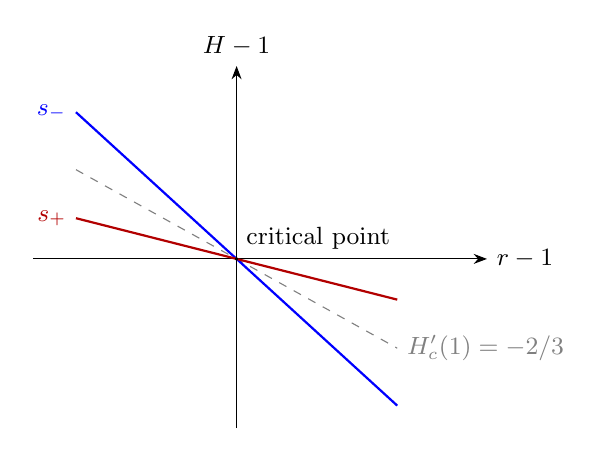
\begin{tikzpicture}[x=6cm,y=5cm,>=Stealth,font=\small]
\draw[->] (-.43,0)--(.53,0) node[right] {$r-1$};
\draw[->] (0,-.43)--(0,.49) node[above] {$H-1$};
\draw[gray,dashed] (-.34,.2267)--(.34,-.2267);
\draw[blue,thick] (-.34,.3726)--(.34,-.3726);
\draw[red!70!black,thick] (-.34,.1034)--(.34,-.1034);
\fill (0,0) circle[radius=.7pt];
\node[above right] at (0,0) {critical point};
\node[blue,left] at (-.34,.3726) {$s_-$};
\node[red!70!black,left] at (-.34,.1034) {$s_+$};
\node[gray,right] at (.34,-.2267) {$H_c'(1)=-2/3$};
\end{tikzpicture}

\small Tangent-direction schematic at $c=-7$. Lines indicate the two exact
slopes and the tangent to $D=0$, $H_c(r)=r^{-2/3}$; they are not computed
solution profiles, certified intervals, or trajectories in physical time.
\end{center}

The comparison with flat-bed water flow is precise. At the same water state,
removing the bed slope gives $N=7/4\ne0$ while $D=0$, preventing a $C^1$
profile through that state. In the coupled model $P=7/4$ cancels this defect
and simultaneously satisfies Exner. This is not a singular $G\to0$ limit,
and not a claim that every flat-bed critical point is nonsmooth. The exact
critical state has $\mathrm{Fr}_{\rm rad}^2=1$ but
$\mathrm{Fr}_{\rm total}^2=5/4$.

\section{Scope boundaries, counterchecks and review map}
Chesnokov's model is water flow above a fixed flat bottom
\cite[p.~1, Eq.~(1.1)]{chesnokov}; its stationary ring formulas and the
unbounded derivatives at the discussed critical boundaries appear on
pp.~13--14, Eqs.~(5.1)--(5.2). Its water constants and radial critical condition
are predecessors. The theorem here includes a dynamically coupled slope law,
an Exner-compatible nonzero drift, a saddle-based smooth spatial continuation,
and full-PDE reconstruction. Berthon et al.~\cite[pp.~184--185]{berthon}
already supplies a distinct one-dimensional steady-water/drifting-bed
precedent. These comparisons establish a difference from the inspected
sources, not global priority. The stable-manifold mechanism is classical.

Necessary exclusions and negative cases remain explicit:
\begin{itemize}
\item $r=0$ loses the selected orbit chart; $H=0$ loses the wet-state chart.
\item $C_1=0$ gives $V=0$ on this chart. Tangential momentum then imposes
      no equation on $W$, so deriving its integral by division is invalid.
      This does not assert nonexistence of zero-radial-flow solutions.
\item $G=0$ or $S=0$ loses the constitutive slope inverse. These require a
      different reduction and are not limits covered by the theorem.
\item At $D=0,N\ne0$ there is no $C^1$ profile through that state.
      Compatibility $D=N=0$ alone is insufficient: in the displayed family,
      $c=0$ gives discriminant $-1539/25<0$ for the unscaled slope
      equation~\eqref{eq:slopes} (or $-1539$ after multiplication by five).
\item At $c=-77/12$ the saddle determinant vanishes. The theorem makes no
      assertion for that zero-eigenvalue point, non-saddles, nonsmooth gluing,
      shocks, dry interfaces, global connections or arbitrary data.
\end{itemize}

The slope-dependent Exner equation is second order in $B$. Therefore the
hydraulic pivot $D=0$ is not asserted to be the characteristic determinant
of the full mixed-order PDE. Locality gives an unspecified sufficiently
small interval; a quantified interval or learned-solution certificate needs
additional validated computation. No ML experiment is claimed in this note.

\begin{center}\small
\begin{tabularx}{\textwidth}{@{}lX@{}}\toprule
Review obligation&Evidence supplied\\\midrule
No prescribed profile in discovery&56 unknown point coefficients; original evolution operators and unsplit determining identities\\
Derived quotient&Exact invariant nullspaces, selected returned subalgebra, bracket and nonzero adapted Jacobian\\
No lost constants/divisors&Original radial currents, integrating factor, $C_1,C_2,C_3$, bed gauge and zero-pivot ledger\\
Existence and local coverage&Theorem~\ref{thm:main}, using cited stable-manifold results and a $C^1$ converse argument\\
Full model reconstruction&Direct Cartesian differentiation, including the Exner second derivatives and a bed-slope fault injection\\
Parameter coverage&Exact inequality $c<-77/12$ and Corollary~\ref{cor:persist}\\
Unresolved claims&Priority, empirical applicability, quantified radius/error, full Lie classification and general PDE data\\\bottomrule
\end{tabularx}
\end{center}

\begin{thebibliography}{9}
\bibitem{teschl} G.~Teschl, \emph{Ordinary Differential Equations and Dynamical
Systems}, AMS, 2012. The consulted artifact is the author's preliminary
version distributed with AMS permission, not asserted byte-identical to the
printed edition. Theorems 9.4--9.5: printed p.~259, PDF p.~270;
Theorem 9.6: printed p.~260, PDF p.~271.
\url{https://www.mat.univie.ac.at/~gerald/ftp/book-ode/ode.pdf}.
\bibitem{chesnokov} A.~Chesnokov, \emph{Symmetries and exact solutions of the
rotating shallow water equations}, arXiv:0808.1490v1, 2008.
\url{https://arxiv.org/pdf/0808.1490v1}.
\bibitem{berthon} C.~Berthon, S.~Cordier, O.~Delestre and M.-H.~Le,
\emph{An analytical solution of the shallow water system coupled to the
Exner equation}, C.~R.~Math. 350 (2012), 183--186.
\url{https://doi.org/10.1016/j.crma.2012.01.007}.
\end{thebibliography}
\end{document}
